When exposed to naturalistic stimuli (e.g. movie watching or simulated driving), subjects' experience is closer to their every-day life than with classical
psychological experiments.
% 
This makes naturalistic paradigms an attractive class of
stimulation protocols for brain imaging.
%
However, such stimulations are difficult to quantify, therefore the statistical analysis of the data using supervised regression-based approaches is challenging.
This has motivated the use of unsupervised learning methods that do not make
assumptions about what triggers brain activations in the stimuli.

In this chapter, we first present \emph{independent component analysis} (ICA), a widely used
unsupervised method for neuro-imaging studies routinely applied on individual
subject electroencephalography (EEG)~\cite{makeig1996independent},
magnetoencephalography (MEG)~\cite{vigario1998independent} or functional MRI
(fMRI)~\cite{mckeown1998independent} data, then we review \emph{multiview} unsupervised 
techniques that leverage the availability of data from multiple subjects
performing the same experiments. 

\section{Independent component analysis}
ICA models a set of signals as the product of a \emph{mixing matrix} and a
\emph{component} matrix containing independent components. As will be seen in this
section, the required assumptions on the independent components to guarantee
identifiability are rather weak making ICA a method of choice to analyze the
data of subjects exposed to a stimuli that is difficult to quantify.

ICA is applied in fMRI data to analyze resting state
data~\cite{beckmann2005investigations} or when subjects are
exposed to natural~\cite{malinen2007towards}~\cite{bartels2005brain} or complex stimuli~\cite{calhoun2002different}. 
In M/EEG processing, it is widely used to isolate acquisitions artifacts from neural signal~\cite{jung1998extended}, and to identify brain components of interest~\cite{vigario2000independent, delorme2012independent}.

\subsection{Principal component analysis (PCA)}
- Unicity of SVD
- Complexity of SVD
In ICA, the mixing matrices are assumed to be square. In practice, however we
might want to estimate fewer components that they are observations. Therefore, a
typical pre-processing step is to reduce the dimension by principal component
analysis (PCA). 


For completeness, we start by describing PCA. For a zero-mean data matrix $X$ of size $p\times n$ with $p \leq n$, we denote $X= UD V^{\top}$ the singular value decomposition of $X$ where $U \in \bbR^{p\times p}$, $V \in \bbR^{n \times p}$ are orthogonal and $D$ the diagonal matrix of singular values ordered in decreasing order.
% 
The PCA of $X$ with $p$ components is $Y\in\bbR^{p\times n}$ containing the first $p$ rows of $DV^{\top}$, and it does not hold in general that $YY^{\top}=I_p$: for the rest of the paper, what we call PCA does not include whitening of the signals.


\subsection{Non Gaussian ICA}
\subsubsection{Identifiability}
\subsubsection{Robustness to density missmatch}
\subsubsection{Stability (extended infomax)}
\subsection{non-stationary ICA}
\subsubsection{Identifiability}
\subsubsection{Joint diagonalization objective}
\subsection{Dimension reduction}
So far, we have assumed that the dimensionality of the data $v$ and the number
of components $p$ is the same. 
In practice, however, we might want to estimate fewer components than there are observations per view; the original dimensionality of the data %(number of voxels, sensors) 
might in practice not be computationally tractable.

% The problem of how to perform subject-wise dimensionality reduction in group studies 
% % of data for each of the individuals while still considering them jointly and preserving the signal shared across them
% is an interesting one \emph{per se}, and out of the main scope of this work. For our purposes, it can be considered as a preprocessing step for which well-known various solutions can be applied. % step prior to the application of our method,. 
% We discuss this further in section~\ref{sec:rel_work} and in appendix~\ref{sec:app_rel_work}.

A classical approach to perform dimension reduction is principal component
analysis (PCA) which we now present.
Our data is represented as a random vector $\xb \in \bbR^v$ that is assumed
centered ($\EE[\xb] = 0$). Take $C = \Cov(\xb) \in \mathbb{R}^{v \times v}$ the
covariance of $\xb$ and compute an eigenvalue decomposition $VD^2V {\top} = C$
such that the coefficients of the diagonal matrix $D^2 \in \mathbb{R}^{v
  \times v}$ are ordered in decreasing order and $V$ is an orthogonal matrix.
Then $V = [\vb_1 \dots \vb_m]$ gives the projection vectors such that the $p$ first
principal components are then given by $[\vb_1 \dots \vb_p]^{\top} \xb$. Note
that our formulation of PCA does not include whitening of the signals.



% For a zero-mean data matrix $X$ of size $p\times n$ with $p \leq n$, we denote $X= UD V^{\top}$ the singular value decomposition of $X$ where $U \in \bbR^{p\times p}$, $V \in \bbR^{n \times p}$ are orthogonal and $D$ the diagonal matrix of singular values ordered in decreasing order.
% The PCA of $X$ with $k$ components is $Y\in\bbR^{k\times n}$ containing the
% first $k$ rows of $DV^{\top}$, and it does not hold in general that
% $YY^{\top}=I_k$: in this thesis, what we cann PCA does not include whitening of the signals.
\section{Analysis of MultiView data}
In this section, we present multiview unsupervised techniques suited to
analyze the data of multiple subjects exposed to the same complex stimuli. Such
techniques assume some similarity between the data of different subjects. This
assumption can be justified by the findings of \cite{hasson2004intersubject} showing that brains exposed to the same natural stimuli exhibit synchronous activity.
The task of finding common patterns or responses that are shared between
subjects is called \emph{shared response modeling}.


Many methods for data-driven multivariate analysis of neuroimaging group studies have been proposed. We summarize the characteristics of some of the most commonly used ones.
\subsection{Group independent component analysis}
\label{sec:groupica}
Given the success of ICA in analyzing the data of one subject. It is natural to
look for extensions of ICA in a multiview setting.
However, unlike with univariate methods like the GLM model, statistical inference about multiple subjects using ICA is not straightforward: so-called group-ICA is the topic of various studies~\cite{hyvarinen2013independent}.

Several works assume that the subjects share a common mixing matrix, but with different components~\cite{pfister2019robustifying}~\cite{svensen2002ica}.
% 
Instead, we focus on models where the subjects share a common components matrix, but have different mixing matrices.
When the subjects are exposed to the same stimuli, the common component matrix corresponds to the group \emph{shared responses}.

\subsubsection{CanICA and ConcatICA}
\label{sec:canicaandconcatica}
Most methods proposed in this framework proceed in two steps~\cite{calhoun2009review, huster2015group}.
% 
First, the data of individual subjects are aggregated into a single dataset, often resorting to dimension reduction techniques like Principal Component Analysis (PCA).
% 
Then, off-the-shelf ICA is applied on the aggregated dataset.
% 
This popular method has the advantage of being simple and
straightforward to implement since it resorts to customary single-subject
ICA method.

% 
\cite{varoquaux2009canica}
When datasets are high-dimensional, a three steps procedure is often used: first dimensionality reduction is performed on data of each subject  separately; then the reduced data are merged into a common representation; finally, an ICA algorithm is applied for shared components extraction. The merging of the reduced data is often done by PCA \cite{calhoun2001method} or multi set CCA \cite{varoquaux2009canica}.

% Note that even with large datasets, it can still be computationally feasible to do group level reduction in one step (see \cite{chen2015reduced} or \cite{smith2014group}).
This is a popular method for fMRI~\cite{calhoun2009review} and EEG~\cite{eichele2011eegift} group studies.
These methods directly recover only group level, shared components; when individual components are needed, additional steps are required (back-projection \cite{calhoun2001method} or dual-regression \cite{beckmann2009group}).
% 

\subsubsection{Matching individual ICA decompositions}
\label{sec:permica}
A different path to multi-subject ICA is to extract independent components with individual ICA in each subject and align them. We propose a simple baseline approach to do so called \emph{PermICA}.
Inspired by the heuristic of the hyperalignment method~\cite{haxby2011common} we choose a reference subject and first match the components of all other subjects to the components of the reference subject. The process is then repeated multiple times, using the average of previously aligned components as a reference. Finally, group components are given by the average of all aligned components. We use the Hungarian algorithm to align pairs of mixing matrices~\cite{tichavsky2004optimal}.

% 
Alternative approaches involving clustering have also been developed~\cite{esposito2005independent,bigdely2013measure}.
\subsubsection{Likelihood based method}
\label{sec:guo}
One can consider the more general model $\xb_i = A_i\sbb^i + \nb_i$, where the noise covariance can be learned from the data~\cite{guo2008unified}.
% 
Having the simpler model~\eqref{eq:mvica:model} leads to a closed-form likelihood, that can then be optimized by more efficient means than the EM algorithm.
In model~\eqref{eq:mvica:model}, the noise can be interpreted as individual variability rather than sensor noise. %It offers a way to capture more structured noise as is often the case in brain signals.
% It offers a way to capture more structured noise, which is often present in neuroimaging recordings~\cite{engemann2015automated}.

\subsection{Independent vector analysis}
Independent vector analysis~\cite{lee2008independent} (IVA) models the data as a linear mixture of independent components $\xb_i = A_i \sbb_i$ where each component $s_{ij}$ of a given view $i$ can depend on the corresponding component in other views ($(s_{ij})_{i=1}^m$ are not independent).
\label{sec:IVA}
Practical implementations of this very general idea assume a distribution for $p((s_{ij})_{i=1}^m)$. In IVA-L~\cite{lee2008independent}, $p((s_{ij})_{i=1}^m) \propto \exp(-\sqrt{\sum_i (s_{ij})^2})$ (so the variance of each component in each view is assumed to be the same), in IVA-G~\cite{anderson2011joint} or in~\cite{via2011maximum}, $p((s_{ij})_{i=1}^m) \sim \mathcal{N}(0, R_{ss})$ and~\cite{engberg2016independent} proposed a normal inverse-Gamma density.
\subsubsection{IVA-L}
\subsubsection{IVA-G}

\subsection{Multiset CCA}
\label{sec:mcca}
In its basic formulation, CCA identifies a shared space between two datasets.
The extension to more than two datasets is ambiguous, and many
different generalized CCA methods have been proposed. \cite{kettenring1971canonical} introduces 6 objective functions that reduce to CCA when $m=2$ and \cite{nielsen2002multiset} considered 4 different possible constrains leading to 24 different formulations of Multiset CCA.

In this section, we present the formulation refered to
in~\cite{nielsen2002multiset} as SUMCORR with constraint 4 which is one of the
fastest to fit.

\subsection{Hyperalignment}

\subsection{The shared response model (SRM)}
The shared response model~\cite{chen2015reduced} is a multi-view latent factor
model. The data $\xb_1 \dots \xb_m$ are modeled as random vectors following the model:
\begin{align}
 &\xb_i = A_i \sbb + \nb_i \\
  &A_i^{\top}A_i = I_p
  \label{eq:model:srm}
\end{align}
where $\xb_i \in \RR^v$ is the data of view $i$, $A_i \in \RR^{p, v}$ is the
mixing matrix of view $i$, $\nb_i$ is the noise of view $i$ and $\sbb$ are the
shared components referred to as the \emph{shared response} in fMRI applications.
The mixing matrices
$A_i$ are assumed to be orthogonal so that $A_i^{\top}A_i = I_p$. However in
general the matrix $A_i A_i^{\top}$ is different from identity. The noise
$\nb^i$ is assumed to be Gaussian with covariance $\Sigma_i$ and independent
across views. We assume the number of features $v$ to be much larger than the
number of components $p$: $v >> p$.

The conceptual figure~\ref{fig:srm:conceptual_figure} illustrates an 
application of the shared response model to fMRI data. The mixing
matrices are spatial topographies specific to each subjects while the shared
components give the common timecourses.

\begin{figure}
  \centering
  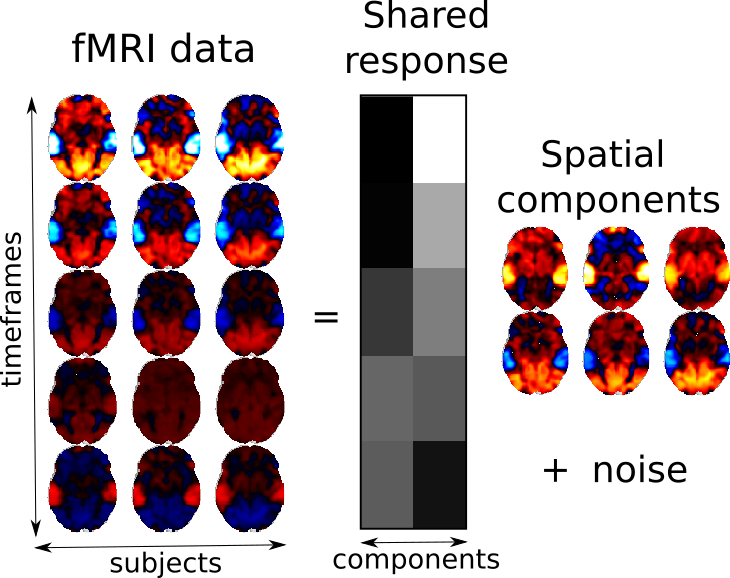
\includegraphics[scale=0.3]{figures/srm/conceptual_figure31.png}
  \caption{\textbf{Shared response model}: The raw fMRI data are modeled as a weighted combination of subject-specific spatial components with additive noise. The weights are shared between subjects and constitute the shared response to the stimuli.}
  \label{fig:srm:conceptual_figure}
\end{figure}

In~\cite{chen2015reduced, anderson2016enabling}, two versions of the shared response model are
introduced which we now present.
\subsubsection{Deterministic shared response model}
\label{sec:deterministicsrm}
The deterministic shared response model sees both $A_i$ and $\sbb$ as parameters to be
estimated and $\forall i, \Sigma_i=\sigma^2 I_v$ where $\sigma$ is an hyper-parameter.
The model is optimized by maximizing the log-likelihood.
The likelihood is given by: $p(\xb) = \prod_i \Ncal(\xb_i; A_i \sbb, \sigma^2 I)$ and
therefore the negative log-likelihood is given up to a constant independent of
$A_i$ and $\sbb$ by:
\begin{align}
  \loss = \sum_i \|A_i \sbb - \xb_i \|^2 = \| \sbb \|^2 -2 \langle A_i \sbb, \xb_i \rangle + \| \xb_i \|^2
  \label{eq:detsrmloss}
\end{align}
The negative log-likelihood $\loss$ is optimized by performing alternate minimization on $(A_1 \dots A_m)$
and $\sbb$. Note that the hyper-parameter $\sigma$ does not have an influence on
the loss and can therefore be safely ignored.

The gradient with respect to $\sbb$ is given by $ \sum_i A_i^{\top}(A_i \sbb -
\xb_i) = \sum_i (\sbb -
A_i^{\top} \xb_i)$
yielding the closed form updates:
\begin{equation}
  \sbb \leftarrow  \frac1m \sum_i (A_i^{\top} \xb_i)
  \label{eq:srm:supdate}
\end{equation}

From \eqref{eq:detsrmloss}, minimizing $\loss$ with respect to $A_i$ is
equivalent to maximize $\langle A_i, \xb_i \sbb^{\top} \rangle$ and therefore we
have:
\begin{equation}
  A_i \leftarrow  \Pcal(\xb_i \sbb^T)
  \label{eq:detsrm:Aiupdate}
\end{equation}
where $\Pcal$ is the projection on the Stiefel manifold: $\Pcal(M) = M
(M^{\top}M)^{-\frac12}$. In practice $\Pcal(M)$ is computed by performing an SVD
of $M$, $M = U_M D_M V_M^{\top} $ so that $\Pcal(M) = U_M V_M^{\top}$.

The complexity of Deterministic SRM is in $\bigO(\mathrm{n_{iter}} mpvn)$ where
$n$ is the number of samples and $\mathrm{n_{iter}}$ the number of iterations.
We monitor the convergence by looking at the $\ell_{infty}$ norm of the
gradient. We can monitor the gradient without any increase in complexity.
Indeed, after the updates with respect to each mixing matrix have been
carried, only the gradient with respect to $\sbb$ remains: $\sum_i
(\sbb - A_i^{\top}\xb_i)$. The algorithm is stopped when the
gradient is below a chosen tolerance.

\subsubsection{Probabilistic SRM}
\label{sec:probabilisticsrm}
In Probabilistic SRM , $\Sigma_i=\sigma_i^2 I_v$ and the shared
components are assumed to be Gaussian $\sbb \sim \Ncal(0, \Sigma_s)$.
In~\cite{chen2015reduced}, $\Sigma_s$ is only assumed to be definite positive. However,
as will be seen in the FastSRM chapter, enforcing a diagonal $\Sigma_s$ ensures
identifiability (provided the diagonal values are different). So we assume for
now on, that $\Sigma_s$ is diagonal.

The model is optimized via the expectation maximization algorithm.
Denoting $\VV[\sbb | \xb] = (\sum_i \frac1{\sigma_i^2} I +
\Sigma_s^{-1})^{-1}$ and $\EE[\sbb | \xb] = \VV[\sbb | \xb] \sum_i \frac1{\sigma_i^2}
A_i^{\top}\xb_i$, we have
\begin{align}
  p(\xb, \sbb) &= \prod_i \frac{\exp(-\frac{\|\xb_i - A_i \sbb \|^2}{2 \sigma_i^2})}{(2 \pi \sigma_i^{2v})^{\frac12}} \frac{\exp(-\frac12 \langle \sbb , \Sigma_s^{-1} \sbb \rangle )}{(2 \pi | \Sigma_s|)^{\frac12}} \\
               &= c_1 \exp(-\frac12 \left( \sum_i \frac1{\sigma_i^2}\|\xb_i\|^2 - 2  \langle \sum_i \frac1{\sigma_i^2} A_i^{\top}\xb_i, \sbb \rangle \right. \\& \left.+ \sum_i \frac1{\sigma_i^2} \| \sbb \|^2 + \langle \sbb, \Sigma_s^{-1} \sbb \rangle  \right)) \\
               &= c_2 \exp(-\frac12 \left( \langle  \sbb - \EE[\sbb | \xb], \VV[\sbb | \xb]^{-1} ( \sbb - \EE[\sbb | \xb])  \rangle \right)) \label{probsrmcompleted}
\end{align}
where $c_1 = \frac1{(2 \pi \sigma_i^{2v})^{\frac12}}\frac1{(2 \pi |
  \Sigma_s|)^{\frac12}}$ and $c_2 = c_1 \exp(-\frac12( \sum_i
\frac1{\sigma_i^2}\|\xb_i\|^2 - \langle  \EE[\sbb | \xb], \VV[\sbb | \xb]^{-1} \EE[\sbb | \xb] \rangle))$ are independent of $\sbb$.
Therefore $\sbb| \xb \sim \Ncal(\EE[\sbb | \xb], \VV[\sbb, \xb])$

The negative completed log-likelihood is given by
\begin{align}
	\loss = \sum_i \frac12 v \log(\sigma_i^2) + \frac1{2 \sigma_i^2} \| \xb_i - A_i \sbb \|^2
\end{align}
updates are therefore given by:
\begin{align}
&\sigma_i^2 \leftarrow \frac1{v} (\| \xb_i - A_i \EE[\sbb|\xb]\|^2 + \| \diag(\VV[\sbb | \xb]) \|^2) \\
  &A_i \leftarrow \Pcal(\xb_i \EE[\sbb|\xb]^{\top}) \\
  & \Sigma_s \leftarrow \VV[\sbb | \xb] + \EE[\sbb | \xb] \EE[\sbb | \xb]^{\top}
    \label{eq:srm:Aiupdate}
\end{align}

It is useful to access the log-likelihood to check the implementation of the
algorithm and monitor the convergence. From equation~\eqref{probsrmcompleted},
the likelihood is given by:
\begin{align}
  p(\xb) &= c_2 \int_{\sbb} \exp(-\frac12 \left( \langle  \sbb - \EE[\sbb | \xb], \VV[\sbb | \xb]^{-1} ( \sbb - \EE[\sbb | \xb])  \rangle \right)) d\sbb \\
         &= c_2 (2 \pi |\VV[\sbb | \xb]|)^{\frac12}
\end{align}
and so up to constants the negative log-likelihood is given by:
\begin{align}
  -\log(p(\xb)) = &\sum_i \frac{v}{2} \log(\sigma_i^2) + \frac12 \log(|\Sigma_s|) - \frac12 \log(|\VV[\sbb | \xb]|) \\ &+ \sum_i
  \frac12 \frac1{\sigma_i^2}\|\xb_i\|^2 - \frac12 \langle  \EE[\sbb | \xb], \VV[\sbb | \xb]^{-1} \EE[\sbb | \xb] \rangle
\end{align}

The complexity of Probabilistic SRM is $\bigO(\mathrm{n_{iter}} mpvn)$, the same as in
Deterministic SRM.
We can monitor the convergence by looking at the log-likelihood decrease at each iteration
and stop the algorithm when the magnitude of the decrease is below some
tolerance.
The storage requirements of Deterministic or Probabilistic SRM are in
$\bigO(mvn)$ which simply means that the dataset needs to hold in memory.

% \section{Related Work}
% \label{sec:rel_work}
% %

% %
% %

% %
% %
% %

% \textbf{Structured mixing matrices} One strength of our model is that we only assume that the mixing matrices are invertible and still enjoy identifiability whereas some other approaches impose additional constraints. For instance tensorial methods~\cite{beckmann2005tensorial} assume that the mixing matrices are the same up to diagonal scaling.
% %
% Other methods impose a common mixing matrix~\cite{cong2013validating, grin2010independent, calhoun2001fmri, Monti18UAI}. Like PCA, the Shared Response Model~\cite{chen2015reduced} (SRM) assumes orthogonality of the mixing matrices. While the model defines a simple likelihood and provides an efficient way to reduce dimension, the SRM model is not identifiable as shown in appendix~\ref{sec:app_identifiability}, and the orthogonal constraint may not be plausible.
% %

% \textbf{Matching components a posteriori} A different path to multi-subject ICA is to extract independent components with individual ICA in each subject and align them. We propose a simple baseline approach to do so called \emph{PermICA}.
% Inspired by the heuristic of the hyperalignment method~\cite{haxby2011common} we choose a reference subject and first match the components of all other subjects to the components of the reference subject. The process is then repeated multiple times, using the average of previously aligned components as a reference. Finally, group components are given by the average of all aligned components. We use the Hungarian algorithm to align pairs of mixing matrices~\cite{tichavsky2004optimal}.
% %
% Alternative approaches involving clustering have also been developed~\cite{esposito2005independent,bigdely2013measure}.

% \textbf{Deep Learning} Deep Learning methods, such as convolutional auto-encoders (CAE), can also be used to find the subject specific unmixing~\cite{chen2016convolutional}. While these nonlinear extensions of the aforementioned methods are interesting, these models are hard to train and interpret. In the experiments on fMRI data in appendix~\ref{appendix_reproduce}, we obtain better accuracy with MultiView ICA than that of CAE reported in~\cite{chen2016convolutional}.

% \textbf{Correlated component analysis} Other methods can be used to recover the shared neural responses such as the correlated component approach of Dmochowski~\cite{dmochowski2012correlated}. We benchmark our method against its probabilistic version~\cite{kamronn2015multiview} called BCorrCA in Figure~\ref{fig:meg}. Our method yields much better results. 

% \textbf{Autocorrelation} Another way to perform ICA is to leverage spectral diversity of the components rather than non-Gaussianity.
% %
% These methods are popular alternative to non-Gaussian ICA in the single-subject setting~\cite{tong1991indeterminacy, belouchrani1997blind, pham1997blind} and they output significantly different components than non-Gaussian ICA~\cite{delorme2012independent}.
% %
% Extensions to multiview problems have been proposed~\cite{lukic2002ica, congedo2010group}.